%; whizzy chapter -dvi
% -initex iniptex -latex platex -format platex -bibtex jbibtex -fmt fmt
% 以上 whizzytex を使用する場合の設定。
 
%     Tokyo Debian Meeting resources
%     Copyright (C) 2012 Junichi Uekawa
%     Copyright (C) 2011, 2015 Nobuhiro Iwamatsu

%     This program is free software; you can redistribute it and/or modify
%     it under the terms of the GNU General Public License as published by
%     the Free Software Foundation; either version 2 of the License, or
%     (at your option) any later version.

%     This program is distributed in the hope that it will be useful,
%     but WITHOUT ANY WARRANTY; without even the implied warranty of
%     MERCHANTABILITY or FITNESS FOR A PARTICULAR PURPOSE.  See the
%     GNU General Public License for more details.

%     You should have received a copy of the GNU General Public License
%     along with this program; if not, write to the Free Software
%     Foundation, Inc., 51 Franklin St, Fifth Floor, Boston, MA  02110-1301 USA

%  preview (shell-command (concat "evince " (replace-regexp-in-string "tex$" "pdf"(buffer-file-name)) "&"))

%%ここからヘッダ開始。

\documentclass[mingoth,a4paper]{jsarticle}
\usepackage{monthlyreport}
% 日付を定義する、毎月変わります。
\newcommand{\debmtgyear}{2017}
\newcommand{\debmtgmonth}{1}
\newcommand{\debmtgdate}{21}
% started from zero:
% (let ((year 2013) (month 7)) (+ (* (- year 2005) 12) month -1))
\newcommand{\debmtgnumber}{147}

\begin{document}

\begin{titlepage}
\thispagestyle{empty}
% タイトルページ:編集必要な部分は最初のマクロに飛ばすこと

\vspace*{-2cm}
第\debmtgnumber{}回 東京エリア Debian 勉強会資料\\
\hspace*{-2cm}
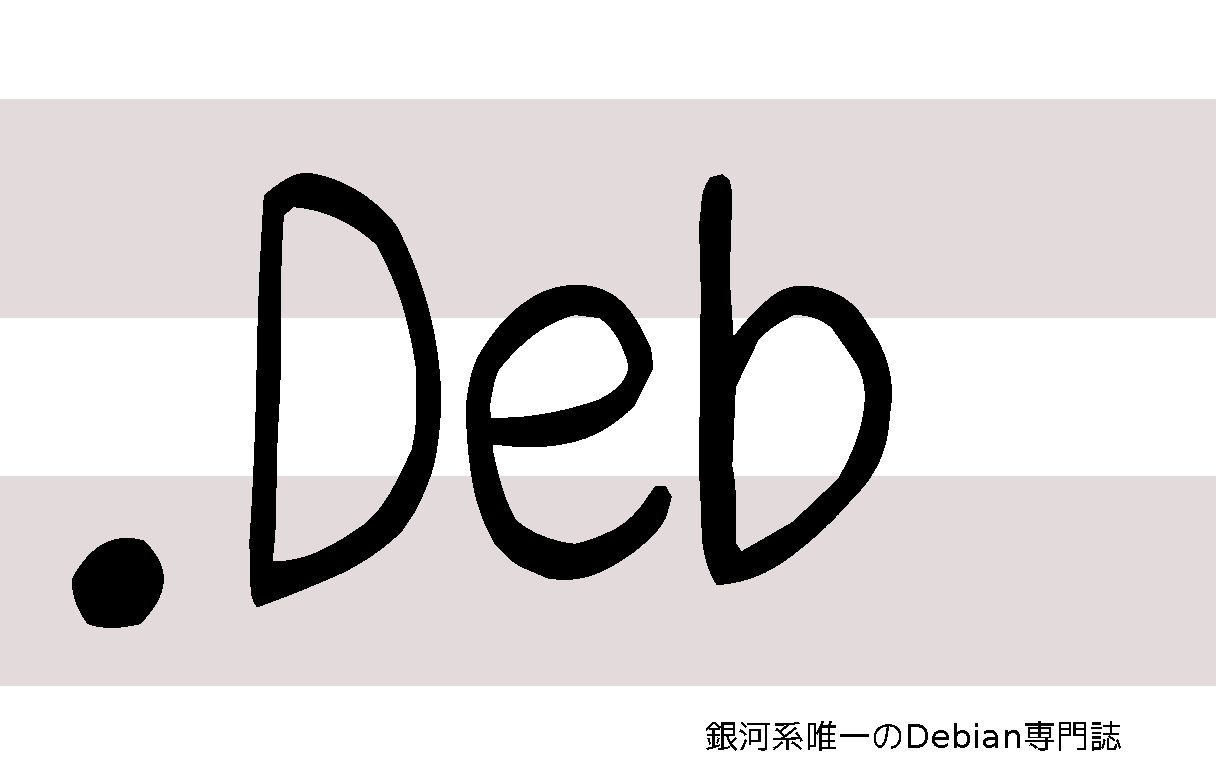
\includegraphics{image2012-natsu/dotdeb.pdf}\\
\hfill{}\debmtgyear{}年\debmtgmonth{}月\debmtgdate{}日

% ここはアップデートすること
% 全角文字にしないとフォントのサイズが合わないので注意
\rotatebox{10}{\fontsize{30}{30} {\gt 特集 :debhelper 10}}\\

\vspace*{-2cm}
\hfill{}
\includegraphics[height=6cm]{image200502/openlogo-nd.eps}
\end{titlepage}

\newpage

\begin{minipage}[b]{0.2\hsize}
 \definecolor{titleback}{gray}{0.9}
 \colorbox{titleback}{\rotatebox{90}{\fontsize{80}{80} {\gt デビアン勉強会} }}
\end{minipage}
\begin{minipage}[b]{0.8\hsize}
\hrule
\vspace{2mm}
\hrule
\begin{multicols}{2}
\tableofcontents
\end{multicols}
\vspace{2mm}
\hrule
\end{minipage}

\dancersection{最近のDebian関連のミーティング報告}{杉本 典充}

\subsection{第146回東京エリアDebian勉強会}

2016年11月19日(土)に第146回東京エリアDebian勉強会を開催しました。会場は銀座にある朝日
ネットさんをお借りして行いました。参加者は5名でした。発表は、yy\_y\_ja\_jpさんによる「dh\_strip\_nondeterminismについて」でした。

発表ではパッケージのビルド時にファイルへ埋め込まれる動的な情報をdebianディレクトリ配下などの情報を用いてビルド後のファイルへ上書きするdh\_strip\_nondeterminismの動作を調べてみたものでした。これはreproduce buildできるようにしようとする取り組みの一環として開発されたとのことです。ファイル形式ごとに書き換えるルールがあり、様々なファイルに対応させるには多くの人の協力が必要に感じました。

勉強会終了後は参加者で懇親を深めました。


\subsection{Mini Debian Conference Japan 2016}

2016年12月10日(土)に"Mini Debian Conference Japan 2016"が開催されました。場所は東京日本橋のサイボウズ様をお借りし、"LibreOffice Kaigi 2016.12"と併催で行いました。

日本だけでなく台湾から発表者として参加した方もおり、一般参加者の方は76名の応募がありました。

発表内容は組み込み、ライセンス、web関連、バーチャルシンガーと多岐に渡る内容でした。

以下URLにwebサイトが公開されており、発表内容を見ることができます。

\url{http://miniconf.debian.or.jp/}


\dancersection{事前課題}{杉本 典充}

今回の事前課題は以下です:
\begin{enumerate}
  \item Hack Timeは何をしますか。
\end{enumerate}
この課題に対して提出いただいた内容は以下です。
\begin{multicols}{2}
{\small
\begin{prework}{ dictoss }
  \begin{enumerate}
  \item stretch$B$N%P%0$D$V$7(B
  \end{enumerate}
\end{prework}

\begin{prework}{ yy\_y\_ja\_jp }
  \begin{enumerate}
  \item DDTSS
  \end{enumerate}
\end{prework}

\begin{prework}{ oguraysu }
  \begin{enumerate}
  \item postfix$B$N@_Dj$r$7$F$_$k(B
  \end{enumerate}
\end{prework}

\begin{prework}{ henrich }
  \begin{enumerate}
  \item $B%&%'%V%5%$%H$N:F9=C[(B
  \end{enumerate}
\end{prework}

\begin{prework}{ upsilon }
  \begin{enumerate}
  \item TrimSlice$B$K(BDebian(armhf)$B$r%$%s%9%H!<%k$7$^$9(B
  \end{enumerate}
\end{prework}

\begin{prework}{ kenhys }
  \begin{enumerate}
  \item $B%Q%C%1!<%8$N%a%s%F%J%s%9(B
  \end{enumerate}
\end{prework}

\begin{prework}{ takaswie }
  \begin{enumerate}
  \item $B8=:_3+H/Cf$N%+!<%M%k%b%8%e!<%k(B(snd-firewire-motu)$B$N:n6H$r$7$^$9!#(B
  \end{enumerate}
\end{prework}

}
\end{multicols}

\dancersection{Debian Trivia Quiz}{杉本 典充}

Debianの昨今の話題についてのQuizです。

今回の出題範囲は\url{debian-devel-announce@lists.debian.org} や \url{debian-news@lists.debian.org}に投稿さた内容などからです。

\begin{multicols}{2}
%; whizzy-master ../debianmeetingresume201311.tex
% $B0J>e$N@_Dj$r$7$F$$$k$?$a!"$3$N%U%!%$%k$G(B M-x whizzytex $B$9$k$H!"(Bwhizzytex$B$,MxMQ$G$-$^$9!#(B
%

\santaku
{Debian 9 (stretch)$B$,(B 2017-01-07$B$K(Bsoft freeze$B$KF~$C$?$3$H$,%"%J%&%s%9$5$l$^$7$?!#(Bsoft freeze$B$K$J$k$H2?$,$G$-$J$/$J$k$G$7$g$&$+!#(B}
{Debian Wiki$B$N(Bstretch$B%Z!<%8$NJQ99(B}
{$B?75,$N%=!<%9%Q%C%1!<%8$N%"%C%W%m!<%I(B}
{$B4{B8$N%=!<%9%Q%C%1!<%8$N%"%C%W%m!<%I(B}
{B}
{soft freeze$B$KF~$k$H4{B8%Q%C%1!<%8$NIJ<A8~>e$KCmNO$;$h!"$H$$$&$3$H$G?75,$N%=!<%9%Q%C%1!<%8$r%"%C%W%m!<%I$G$-$J$/$J$j$^$9!#(Bfull freeze$B$O(B2017-02-05$B$KM=Dj$5$l$F$$$^$9!#%Q%C%1!<%8$,(Bunstable$B$+$i(Btesting$B$X0\9T$9$k$^$G:GC;(B10$BF|4V$+$+$k$?$a!"Aa$a$K=$@5$7$F%"%C%W%m!<%I$7$^$7$g$&!#(B\url{https://lists.debian.org/debian-devel-announce/2017/01/msg00002.html}}

\end{multicols}


% % (query-replace-regexp "<.*?>" "")
% % (query-replace-regexp "^[	 ]\+" "")

%-------------------------------------------------------------------------------
\dancersection{debhepler 10の新機能を確認してみよう}{杉本 典充}
%-------------------------------------------------------------------------------

\subsection{はじめに}

Debian 9(コードネーム「stretch」)のsoft freezeが行われました。そのリリースの中に新しいバージョンであるdebhelper 10が含まれています。

debianパッケージをビルドするツールとして普及しているdebhelperのバージョン10の新機能について調べてみました。


\subsection{debhelperとは}

debhelperとは、debianパッケージを作成するために役に立つツールコマンド群です。debhelperのコマンド群の多くはdhで始まるコマンド名になっています。debhelperのツール群のほとんどはperlで書かれています。

debhelperには大まかに以下の機能があります。

\begin{itemize}
\item パッケージをビルドできるようにdebianディレクトリ配下のファイルを生成、編集するコマンド
  \begin{itemize}
  \item 例:dh\_make\footnote{パッケージをビルドするmakeファイルに相当するdebian/rulesファイルのひな形を作成するコマンド}、dch\footnote{debian/changelogを編集するためEDITORを起動するコマンド}
  \end{itemize}
\item パッケージのビルド処理に利用するコマンド
  \begin{itemize}
  \item 例:dh\footnote{debian/rulesのターゲットにこの1行だけあれば良い場合もある強力なコマンドです}、dh\_clean\footnote{debianパッケージをビルドするために生成するbuildディレクトリや不要なファイルを削除するコマンド}、dh\_install\footnote{ビルド後のパッケージのインストール処理を実行するコマンド}など
  \item 上記コマンドをオーバーライドしてカスタマイズすることができます(例:override\_dh\_clean)
  \end{itemize}
\end{itemize}


\subsection{debhelperの使い方例}


GNUのwebサイトにhelloというお手本プログラムがありますので、これを例にパッケージを作成してみます。debhelperを使ったパッケージのビルドのマニュアルは以下にありますので参考にしてください。


なお、debian/rulesファイルの中身はdebianパッケージ「hello」のファイルを引用しています。

\url{https://www.debian.org/doc/manuals/maint-guide/first.ja.html}

\begin{commandline}
  $ vi ~/.bashrc
  export DEBEMAIL=''dictoss@live.jp''
  export DEBFULLNAME=''Norimitsu Sugimoto''

  $ sudo apt-get install dh-make build-essential

  $ sudo apt-get install autotools-dev
  $ wget https://ftp.gnu.org/gnu/hello/hello-2.10.tar.gz
  $ tar xf hello-2.10.tar.gz
  $ cd hello-2.10
  $ dh_make -f ../hello-2.10.tar.gz
  Type of package: (single, indep, library, python)
  [s/i/l/p]? s
  Email-Address       : dictoss@live.jp
  License             : blank
  Package Name        : hello
  Maintainer Name     : Norimitsu Sugimoto
  Version             : 2.10
  Package Type        : single
  Date                : Thu, 19 Jan 2017 23:13:10 +0900
  Are the details correct? [Y/n/q] Y
  Done. Please edit the files in the debian/ subdirectory now.

  $ ls .. | grep hello
  hello-2.10
  hello-2.10.tar.gz
  hello_2.10.orig.tar.gz

  $ vi debian/changelog
  $ vi debian/control

  $ vi debian/rules
  #!/usr/bin/make -f
  %:
      dh $@

  override_dh_auto_build:
      touch man/hello.1
      dh_auto_build

  override_dh_auto_clean:
      [ ! -f Makefile ] || $(MAKE) distclean

  override_dh_installdocs:
      dh_installdocs NEWS

  $ dpkg-buildpackage -uc -us

  $ ls .. | grep hello
  hello-2.10
  hello-2.10.tar.gz
  hello-dbgsym_2.10-1_amd64.deb
  hello_2.10-1.debian.tar.xz
  hello_2.10-1.dsc
  hello_2.10-1_amd64.buildinfo
  hello_2.10-1_amd64.changes
  hello_2.10-1_amd64.deb
  hello_2.10.orig.tar.gz
\end{commandline}

\subsection{debhelper 10の変更点}

\subsubsection{debian/compat}

debhelperを使ってビルドするパッケージの場合、debian/compatファイルを用意することになっています。

debian/compatファイルにはdebhelperの互換性レベルを記述し、debhelper 10では"10"と記述します。

\begin{commandline}
$ cat debian/compat
10
\end{commandline}


\subsubsection{autoreconfが自動的に実行されるようになった}

debian/compat=10の場合、自動的にautoreconfが実行されるようになりました。

以下はunstable環境のdebhelper-10.2.3において、helloパッケージをビルドしたときに出力するhello\_2.10-1\_amd64.buildをdebian/compat=9の場合とdebian/compat=10の場合の差分を抽出した一部です。dh\_autoreconfを呼び出していることを確認できます。そのため、debian/controlのBuild-Dependsにautoreconfの実行に不足があるとautoreconfでエラーが発生する場合がありますのでビルドログを確認しましょう。

\begin{commandline}
  (省略)
+   dh_autoreconf_clean
    dh_clean
  dpkg-source -b hello-2.10
 dpkg-source: info: using source format '3.0 (quilt)'
@@ -64,6 +23,82 @@
 dh build
    dh_testdir
    dh_update_autotools_config
+   dh_autoreconf
  (省略)
\end{commandline}

  
\subsubsection{Build-Dependsにdh-systemdが不要になった}

debhelper 9まではsystemdの処理を行うパッケージの場合は、Build-Dependsにdh-systemd\footnote{dh\_systemd\_enable、dh\_systemd\_start、systemd2initコマンドをインストールするパッケージ}を含める必要がありました。

debhelper 10ではdh-systemdが取り込まれたため、debian/compat=10の場合はBuild-Dependsにdh-systemdを含める必要がなくなりました。代わりにdebhelperのバージョンを指定する必要があります。

\begin{commandline}
  $ cat debian/compat
  10
  $ cat debian/control
  (省略)
  Build-Depends: debhelper (>= 9.20160709)
  (省略)
\end{commandline}


\subsubsection{parallelオプションが自動的に付与されるようになった}

debian/compat=10の場合、"--parallel"オプションをデフォルトで付与するようになりビルド処理にマルチコアを有効活用するようになりました。debian/compatが9以下の場合は"--parallel"オプションは明示的に指定する必要がありました。

"--parallel"オプションが有効の場合、パッケージのビルド処理を行うdpkg-buildpackageコマンドの"-j"オプション(ジョブ数を指定するパラメータ)を指定するようになります。指定するジョブ数はデフォルトで論理CPUコア数となり、"--max-paralle"オプションで明示的に指定することもできます。

また、複数ジョブを利用したビルドを意図的に行わないようにするには"--no-parallel"というオプションがあります。

\begin{commandline}
#!/usr/bin/make -f
%:
    dh $@ --no-parallel
\end{commandline}

なお、helloパッケージのdebian/rulesは以下のようになっています。

\begin{commandline}
#!/usr/bin/make -f
%:
    dh $@

override_dh_auto_clean:
    [ ! -f Makefile ] || $(MAKE) distclean

override_dh_installdocs:
    dh_installdocs NEWS
\end{commandline}

上記のdebian/rulesでdebian/compat=9の場合とdebian/compat=10の場合のビルドログからジョブ数に何が指定されているか確認します。

ビルドに利用したマシンはHP EliteBook 820 G3でCPUは「Intel(R) Core(TM) i5-6200U CPU @ 2.30GHz」となっています。2コアHyperThreadingありのCPUであり、論理4コアです。以下のビルドログでは、ジョブ数が4になっていることを確認できます。

\begin{commandline}
$ diff -u hello_2.10-1_amd64.build.compat9 hello_2.10-1_amd64.build.compat10 | grep ``make -j''
  -make -j1
  +make -j4
  -make -j1 check VERBOSE=1
  +make -j4 check VERBOSE=1
  -make -j1 install DESTDIR=/home/norimitu/mkdeb/hello-2.10/debian/hello AM_UPDATE_INFO_DIR=no
  +make -j4 install DESTDIR=/home/norimitu/mkdeb/hello-2.10/debian/hello AM_UPDATE_INFO_DIR=no  
\end{commandline}


\subsubsection{dh\_installdebの変更}

debian/compat=10では、dh\_installdebの動作の一部が変更になります。

\subsubsubsection{package.maintscriptの引数がシェル展開されなくなる}

dh\_installdebのpackage.maintscriptの処理時に記述するスクリプトは、シェル変数をエスケープするようになりました。以下はman dh\_installdeb(1)の記述の抜粋です。

\begin{commandline}
  package.maintscript
    Lines in this file correspond to dpkg-maintscript-helper(1) commands and
    parameters.  However, the ``maint-script-parameters'' should not be
    included as debhelper will add those automatically.

    Example:

      # Correct
      rm_conffile /etc/obsolete.conf 0.2~ foo
      # INCORRECT
      rm_conffile /etc/obsolete.conf 0.2~ foo -- "$@"
\end{commandline}

上記の"\$@"の部分がエスケープされるようになりシェル展開されなくなります。そのため、引数にシェル変数やシェルのメタ文字を指定していた場合は意図した文字列に置換されなくなりますので修正が必要になります。


\subsubsubsection{package.shlibsの処理がdh\_makeshlibsで実行するように変更}


debian/compatが9以下の場合は、dh\_installdebの処理でpackage.shlibsを通常/var/lib/dpkg/infoディレクトリ配下にインストールします。

debian/compatが10以降では、dh\_makeshlibsの処理でpackage.shlibsを処理するように変更されました。


\subsection{まとめ}

debhelper 10の新機能についてまとめてみました。stretchにはdebhelper 10が含まれるためこれからパッケージを作成する場合や修正する場合にdebhelper 10へ対応させるとよいと思います。


\subsection{参考文献}

\begin{itemize}
\item debhelper 10 is now available \url{https://nthykier.wordpress.com/2016/09/11/debhelper-10-is-now-available/}
\item man debhelper(7)
\item man dh(1)
\item man dh\_installdeb(1)
\item Debian 新メンテナーガイド \url{https://www.debian.org/doc/manuals/maint-guide/}
\item 「dh-systemdはdebhelper 9.20160709で統合された」 henrich, 2016-08-25 \url{http://qiita.com/henrich/items/e1651e3284c6b3d0d39e}
\end{itemize}


%
% 冊子にするために、4の倍数にする必要がある。
% そのための調整
%\dancersection{メモ}{}
\mbox{}\newpage
\mbox{}\newpage
\mbox{}\newpage


\vspace*{15cm}
\hrule
\vspace{2mm}

\includegraphics[width=2cm]{image200502/openlogo-nd.eps}
\noindent \Large \bf Debian 勉強会資料\\
\noindent \normalfont \debmtgyear{}年\debmtgmonth{}月\debmtgdate{}日 \hspace{5mm}  初版第1刷発行\\
\noindent \normalfont 東京エリア Debian 勉強会 (編集・印刷・発行)\\
\hrule

\end{document}
